%
% Informe interno sobre los datos de Diego Arango
%
\documentclass[a4paper,10pt]{article}
% \documentclass[a4paper,10pt,dvips]{article} 
\usepackage[T1]{fontenc}
\usepackage[utf8]{inputenc}
\usepackage[spanish]{babel}
\usepackage{hyperref}
\usepackage{amsmath}
\usepackage{amssymb}
\usepackage{amsfonts}
%\usepackage{graphicx}
%\usepackage{pstricks}

\setlength{\oddsidemargin}{0pt} \setlength{\evensidemargin}{0pt}
\setlength{\marginparwidth}{1in} \setlength{\marginparsep}{0pt}

\setlength{\topmargin}{0pt} \setlength{\headheight}{0pt}
\setlength{\headsep}{0pt} \setlength{\topskip}{0pt}

%\footheight 0pt
%\footskip 0pt
% A4 is 29,7301778cm x 21,0224103cm
%     =  9,7047944in x 6,2765395in
\setlength{\textheight}{24,6501778cm}
\setlength{\textwidth}{15,9424103cm}

\setlength{\parindent}{0pt}

\pagestyle{plain}

\title{Scatterplot clustering for the integrative analysis of expression and methylation data}
\author{M. Carme Ruiz de Villa, Francesc Carmona \\ Diego Arango del Corro, Alex Sánchez}
\date{2014-09-19}

%
\usepackage{Sweave}

\setkeys{Gin}{width=0.6\textwidth}

\begin{document}
\Sconcordance{concordance:informeMamen.tex:informeMamen.Rnw:%
1 153 1 1 24 1 1 1 9 4 1 1 4 4 1 1 54 1 32 3 1 1 21 6 1 1 14 1 2 4 1 1 %
22 3 1 1 19 1 1 1 13 5 1 1 15 2 1 1 12 5 0 1 3 1 2 4 1 1 38 1 17 3 1 1 %
2 1 0 6 1 5 0 1 1 6 0 1 2 2 1 1 13 4 0 1 12 4 0 1 3 16 1}


\maketitle
\thispagestyle{empty}

\begin{abstract}
En este trabajo se utilizan las técnicas de 
\end{abstract}

\vfill

\begin{center}

\includegraphics{figuras/signatura_cmyk.pdf}
\end{center}

\newpage

\section{Métodos estadísticos}

\subsection{Gene-specific methylation on-off threshold}

Methylation is often described as a binary on-off signal,
and it is widely recognized that methylation represses gene
expression. Typically, if a gene is controlled by its methylation,
its expression is low when methylated. 
On the other hand,
when unmethylated, its expression can be either high or low.
Since measurements for methylation and expression are both
continuous, a biaxial plot of these two signals will exhibit an
L-shape pattern. 

\medskip
If we truly believe that methylation is binary, there are two implications:
\begin{enumerate}
\item the reflection point of the L-shape is an appropriate choice
to binarize methylation data, and
\item conditioning on the
binarized on-off methylation status, the continuous valued
methylation data and expression data should be independent,
\end{enumerate}
which motivates Liu(2012) to quantify the L-shape pattern using
conditional mutual information (MI). 

%In this section, we
%use TCGA data to ask 

\subsection{Conditional Mutual Information}
Two questions: which genes exhibit
L-shape, and what is the optimal threshold for binarizing
methylation data for each L-shape gene.

\medskip
To determine whether methylation and expression of a gene exhibit an L-shape,
we compute the conditional Mutual Information (MI) for different choices of threshold
to binarize the methylation data.


\medskip
If we consider the continuous valued methylation and expression data as two random variables
$X$ and $Y$, and denote a nominal threshold as $t$, the conditional MI can be written as a
weighted sum of MIs on the two sides of the threshold.
\[
\mathit{cMI}(t)=I(X,Y|X>t)P(X>t) + I(X,Y|X\le t)P(X\le t)
\]

\subsection{Optimal threshold}

When $t$ is $0$ or $1$, $\mathit{cMI}$ equals to the mutual information derived 
from all data points.

For an L-shape gene, as $t$ moves from 0 to 1, $\mathit{cMI}(t)$ first decreases and then
increases, and its value approaches zero when $t$ coincides with the reflection point. 
Therefore,

\medskip

The ratio $r=\frac{\min\{\mathit{cMI}(t)\}}{\mathit{cMI}(0)}$ for an L-shape gene is small, 
and $t^{\ast} = \mathrm{argmin}\{ \mathit{cMI}(t) \}$ is the optimal threshold for 
dichotomizing the methylation data of this gene.

\subsection{Joint distribution estimator}
To estimate the MI terms we use a kernel-based estimator, which constructs a joint
probability distribution by applying a Gaussian kernel to each data point, and estimates
the MI based on the joint distribution. The estimator is as follows:
\[
I(X,Y) = \frac 1M \sum_{i=1}^M \log\frac{M\sum_{j=1}^M e^{-\frac{1}{2h^2}((x_i-x_j)^2+(y_i-y_j)^2)}}{%
                                      \sum_{j=1}^M e^{-\frac{1}{2h^2}(x_i-x_j)^2} \sum_{j=1}^M e^{-\frac{1}{2h^2}(y_i-y_j)^2}}
\]
where $h$ is a tuning parameter for the kernel width and empirically set $h=0.3$.
% i and j are indices for samples.
% In our analysis, we normalize the expression data to zero mean.

\subsection{L-shapes}

We filtered for L-shapes using a combination of three criteria:
\begin{itemize}
\item the ratio $r<0.25$
\item unconditioned MI $\mathit{cMI}(0)>0.1$
\item the median expression on the left side of the optimal threshold $t^{\ast}$ is higher
than the median expression on the right side.
\end{itemize}

The parameters are chosen according to a random permutation test (see Liu(2012)).

\medskip
According to the above criteria, a total of 641 genes are selected to be L-shape genes.

\section{El análisis}

\subsection{Los datos}

A partir del archivo \verb|Data_CorrelationsTots.csv| se monta el \verb|data.frame| que contiene los datos.

Una vez limpio y escalados los datos de expresión, se ha grabado el conjunto de datos en el archivo \verb|DataNet.RData| y así podemos cargar los datos directamente.

Las 30 primeras columnas son los datos de Metilación y las últimas 30 son datos de Expresión.

\medskip
En primer lugar procedemos a eliminar de la base de datos aquellos genes que contienen algún valor \textit{missing}. En concreto son 110.
Si los eliminamos quedan 11746 genes remanentes en la base de datos.

\subsection{Cálculo de la \textit{conditional Mutual Information}}

En primer lugar se han creado un par de funciones que calculan la \textit{conditional Mutual Information} entre las muestras de metilación y expresión para cada gen.
Con ellas se procede a la selección de los casos (genes) que verifican los dos primeros criterios.
Los genes que verifican $r<0.25$ son 5040 y los que además verifican que $cMI(0)>0.1$ son 752.

\medskip
A continuación procedemos a seleccionar los genes que han quedado con el tercer criterio.


Dichos genes seleccionados por los tres criterios estan en el archivo \verb|genesSel.RData| y son 643.

\medskip
En el siguiente gráfico vemos un ejemplo de gen seleccionado:
\begin{center}
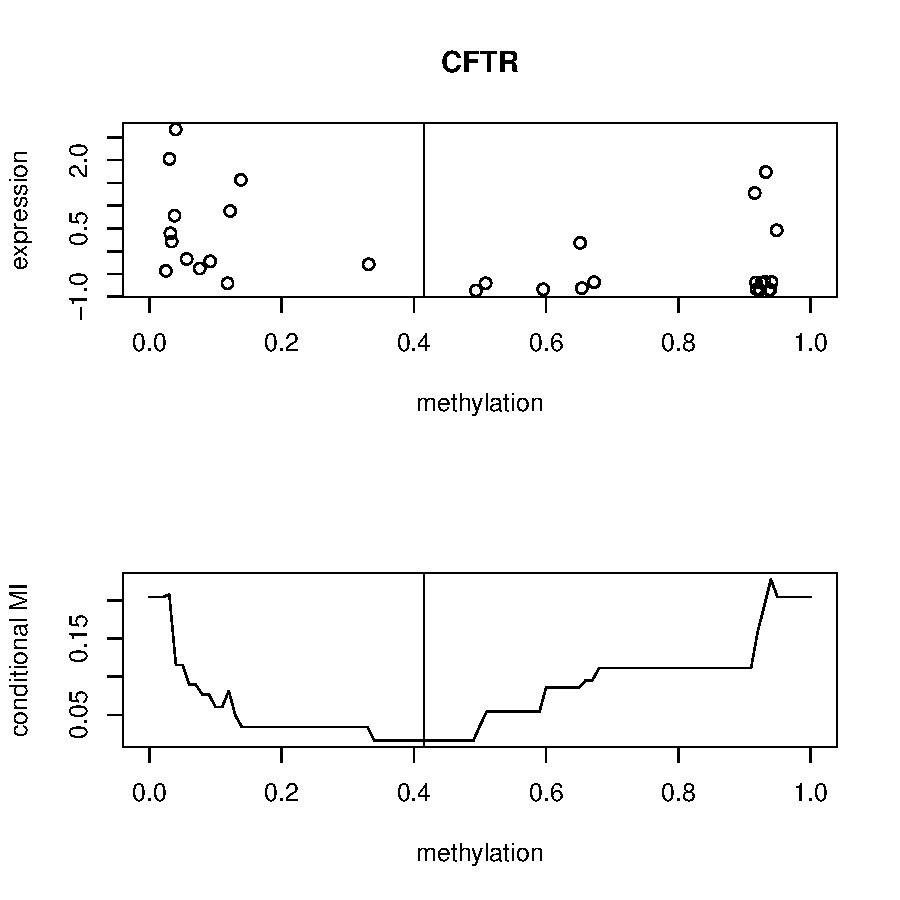
\includegraphics{figuras/-grafic1}
\end{center}

\section{Clustering approach}

Para que el análisis cluster no se pierda con muchos genes que no tienen la forma L deseada, en primer lugar procedemos a eliminar aquellos genes que 
De forma que nos quedamos con 473.

El siguiente paso consiste en calcular las correlaciones de Spearman para cada gen y seleccionar aquellos que tengan una correlación negativa significativa.


Hacemos una lista de matrices met/expr para cada gen. 

\subsection{Análisis cluster}

\subsubsection{Cálculo de los b-splines}

Aplicamos la función \verb|splines| a los datos ajustando con \verb|degree=2| y obtenemos una lista con los coeficientes de los splines de cada gen. 

\subsubsection{Cluster analysis}
Posteriormente se ha realizado un análisis de cluster jerárquico utilizando los coeficientes  de los b-splines como variables para realizar la agrupación. El número de clusters óptimo es 4 con una distribución:
\begin{Schunk}
\begin{Soutput}
Hclustgroups0.5
 1  2  3  4 
94 16 18  3 
\end{Soutput}
\end{Schunk}

Seleccionamos los 4 clusters obtenidos cortando el árbol a 0.5


\begin{center}
La representación de los genes de cada cluster se encuentra  en los ficheros Cluster1...Cluster4 de la carpeta figuras.
\end{center}

Finalmente unimos los genes del cluster 1 y 2 ya que ambos corresponden al patrón de genes regulados por metilación tipo L. 
Para realizar la comparación de ambos métodos realizamos las siguientes intersecciones: Cluster1 con CMI (Tall1) y la unión de Cluster 1 y 2 con CMI (Tall2).
\begin{Schunk}
\begin{Sinput}
> genescluster1 <- names(Hclustgroups[Hclustgroups==1])
> genescluster2 <- names(Hclustgroups[Hclustgroups==2])
> genescriteri3 <- genes.sel
> tall1 <- intersect(genescriteri3,genescluster1)
> tall2 <- intersect(genescriteri3,union(genescluster1,genescluster2))
> gensComuns <- list(tall1=tall1,tall2=tall2)
> length(tall1)
\end{Sinput}
\begin{Soutput}
[1] 75
\end{Soutput}
\begin{Sinput}
> length(tall2)
\end{Sinput}
\begin{Soutput}
[1] 87
\end{Soutput}
\end{Schunk}

El gráfico de los genes de las intersecciones se guardarán en un fichero aparte en la carpeta figuras.

\begin{Schunk}
\begin{Soutput}
pdf 
  2 
\end{Soutput}
\begin{Soutput}
pdf 
  2 
\end{Soutput}
\end{Schunk}

\newpage

\begin{thebibliography}{9}

%\addcontentsline{toc}{chapter}{\numberline{}Bibliografía}

\bibitem{r-project} R Development Core Team (2005). R: A language and environment for statistical computing, 
reference index version 2.14.0. R Foundation for Statistical Computing, Vienna, Austria. ISBN 3-900051-07-0, \\ 
\verb|http://www.R-project.org|




\end{thebibliography}

\end{document}
